\documentclass[12pt]{article}
\usepackage[utf8]{inputenc}
\usepackage{amsmath}
\usepackage{amsfonts}
\usepackage{geometry}
\usepackage{enumitem}
\usepackage{parskip}
\usepackage{hyperref}
\usepackage{graphicx}
\graphicspath{ {./images/} }

\geometry{a4paper, margin=1in}

\title{KCPC Workshop 2 \\ Problems}
\author{}
\date{}

\begin{document}

\maketitle

\section{Psychological Strategies}

\subsection{Pat's Dilemma}
Pat wants to take a 1.5-meter-long sword onto a train, but the conductor won't allow it as carry-on luggage. And the baggage person won't take any item whose greatest dimension exceeds 1 meter. What should Pat do?

\subsection{Thinking in 3D}
We have two polyhedra (i.e., solids with polygonal faces), all of whose edges have length 1: a pyramid with a square base, and a tetrahedron (a tetrahedron is composed of four triangular faces). Suppose we glue the two polyhedra together along a triangular face (so that the attached faces exactly overlap). How many faces does the new solid have?

\section{Wishful Thinking and Make it Easier}

Let $\mathrm{N}$ denote the natural numbers ${1, 2, 3, 4, ...}$. Consider a function $f$ that satisfies $f(1) = 1$, $f(2n) = f(n)$ and $f(2n+1) = 𝑓(2n)+1$ for all $n \in \mathrm{N}$. Find a nice simple algorithm for $f(n)$. Your algorithm should be a single sentence long, at most.

\section{Induction}

Prove that if $n$ is an integer greater than 3, then $n! > 2n$

\section{Draw a Picture}

Once again, you can easily use induction to prove the very cool fact that the sum of the first $n$ perfect cubes is equal to the square of the $n$th triangular number, but can you do it with a picture, instead?

\section{Recast}

Remove the two diagonally opposite corner squares of a chessboard. Is it possible to tile this shape with thirty-one 2×1 “dominos?” (In other words, every square is covered and no dominos overlap.)

\section{Change your Point of View}

What is the first time after 12 o'clock at which the hour and minute hands meet? This is an amusing and moderately hard algebra exercise, well worth doing if you never did it before. However, this problem can be solved in a few seconds \textit{in your head} if you avoid messy algebra and just consider the ``natural'' point of view. Go for it!

\section{Symmetry}

\subsection{Grandma's Cabin}

Your cabin is two miles due north of a stream that runs east-west. Your grandmother’s cabin is located 12 miles west and one mile north of your cabin. Every day, you go from your cabin to Grandma’s, but first visit the stream (to get fresh water for Grandma). What is the length of the route with minimum distance?

\subsection{Geometric}

A square is inscribed in a circle that is inscribed in a square. Find the ratio of the areas of the two squares.

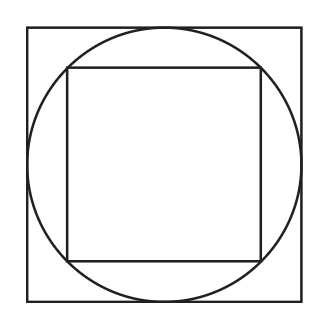
\includegraphics[width=0.3\linewidth]{sym.png}

\subsection{In Probability}
Imagine dropping three pins at random on the unit interval $[0,1]$. They separate the interval into four pieces. What is the average length of each piece? It seems obvious that the answer ``should'' be $1/4$, and this would be true if the probability distributions (mean, standard deviation, etc.) for each of the four lengths are identical.
And indeed, this is true. One way to see this is to imagine that we are not actually dropping three pins on a line segment, but instead dropping four pins on a circle with circumference 1 unit. Wherever the fourth point lands, cut the circle there and ``unwrap'' it to form the unit interval. Ponder this argument until it makes sense. Then try the next few problems!

\begin{itemize}
    \item An ordinary deck of 52 cards with four aces is shuffled, and then the cards are drawn one by one until the first ace appears. On the average, how many cards are drawn?
    \item (Putnam 1992) Four points are chosen at random on the surface of a sphere. What is the probability that the center of the sphere lies inside the tetrahedron whose vertices are at the four points?
\end{itemize}

\section{The Extreme Principle}

Let $B$ and $W$ be finite sets of black and white points, respectively, in the plane, with the property that every line segment that joins two points of the same color contains a point of the other color. Prove that both sets must lie on a single line segment.

\section{Homework}

\subsection{\href{https://atcoder.jp/contests/arc122/tasks/arc122_c}{ARC122, Problem C} -- Calculator}

Snuke has integers $x$ and $y$. Initially, $x=0$, $y=0$.

Snuke can do the following four operations any number of times in any order:

\begin{itemize}
    \item Operation 1: Replace the value of $x$ with $x+1$.
    \item Operation 2: Replace the value of $y$ with $y+1$.
    \item Operation 3: Replace the value of $x$ with $x+y$.
    \item Operation 4: Replace the value of $y$ with $x+y$.
\end{itemize}

You are given a positive integer $N$. Do at most $130$ operations so that $x$ will have the value $N$. Here, $y$ can have any value. And, list out the operations you performed.

We can prove that such a sequence of operations exists under the constraints of this problem.

\subsection{\href{https://atcoder.jp/contests/arc131/tasks/arc131_c}{ARC131, Problem C} -- Zero XOR}

There are $N$ cookies on a desk. Each cookie has a positive integer on its surface: $A_1, A_2, \ldots, A_N$, which are all different.

Let us play a game with two players using these cookies. In this game, the players alternately do the following action:

\begin{quote}
Choose a cookie on the desk and eat it. Then, if the $\text{XOR}$ of the integers written on the remaining cookies on the desk becomes $0$, the player wins, and the game ends.
\end{quote}

You have asked Matthew to play this game with you. You go first, and Matthew goes second. Are you going to win if both players play optimally?

\textit{Hint: You don't need to \textbf{prove} that your solution works rigorously. In competitive programming, getting ``accepted'' \textbf{is} a proof method.}

\end{document}